The Tolerance of some subjects is not representative, as the examiner was not able to apply enough force with the algometer to reach the subjects' Tolerance. These subjects have been excluded. Therefore, the results are based on 32 subjects, 15 subjects in the treatment and 17 subjects in the control group.

\section{Improvements in Threshold and Tolerance}
The mean of the three repetitions of Threshold and Tolerance measurements in each measurement session, Pre and Post, for the treatment and control group with associated standard deviation is illustrated in \tabref{tab:Treatment} and \tabref{tab:Control} respectively. 

\begin{longtable} {l|c|c|c|c|c|c}
	\caption{Threshold and Tolerance, Pre and Post, as well as Improvement (Imp) between these values with associated standard deviation for the treatment group. The mean of those values is indicated in the last row. Inconsistent numbering is due to exclusion of subjects.}
	\label{tab:Treatment} \\
\cellcolor[HTML]{C0C0C0} {} & 
\multicolumn{3}{c|}{ \cellcolor[HTML]{C0C0C0}{\textbf{Threshold}}} & \multicolumn{3}{c}{ \cellcolor[HTML]{C0C0C0}{\textbf{Tolerance}}}  	\\  \rule{0pt}{3ex} 
  \cellcolor[HTML]{C0C0C0}{} &
 \multicolumn{1}{c|}{ \cellcolor[HTML]{C0C0C0}{Pre [kgF]}} & \multicolumn{1}{c|}{ \cellcolor[HTML]{C0C0C0}{Post [kgF]}} &
 \multicolumn{1}{c|}{ \cellcolor[HTML]{C0C0C0}{Imp [\%]}} 
 & \multicolumn{1}{|c|}{ \cellcolor[HTML]{C0C0C0}{Pre [kgF]}} 
 & \multicolumn{1}{c|}{ \cellcolor[HTML]{C0C0C0}{Post [kgF]}} 
 & \multicolumn{1}{c}{ \cellcolor[HTML]{C0C0C0}{Imp [\%]}} 
 	\\ \hline 
\#T1 & 1.84 $\pm$ 0.18 & 1.53 $\pm$ 0.30 & -17.03
& 4.21 $\pm$ 0.25 & 3.93 $\pm$ 0.74 & -6.66\\ \hline
\#T2 & 2.95 $\pm$ 1.02 & 2.85 $\pm$ 0.06 & -3.50 & 7.63 $\pm$ 1.06  & 5.70 $\pm$ 0.87 & -25.26\\ \hline
\#T3 & 2.13 $\pm$ 0.51 & 3.07 $\pm$ 0.29 & 43.75 & 7.75 $\pm$ 0.52 & 8.13 $\pm$ 0.52 & 4.99 \\ \hline
\#T4 & 0.94 $\pm$ 0.15 & 2.34 $\pm$ 0.10 & 148.94 & 3.85 $\pm$ 1.57 & 4.95 $\pm$ 0.24 & 28.55\\ \hline
\#T5 & 1.35 $\pm$ 0.11 & 1.71 $\pm$ 0.35 & 26.11 & 3.11 $\pm$ 0.21  & 3.94 $\pm$ 0.47 & 26.55 \\ \hline	
\#T6 & 0.31 $\pm$ 0.03 & 0.94 $\pm$ 0.18 & 206.52 & 5.95 $\pm$ 1.80 & 5.99 $\pm$  1.02 & 0.67\\ \hline
\#T7 & 2.07 $\pm$ 0.53 & 2.74 $\pm$ 0.41 & 32.15 & 5.44 $\pm$ 0.79 & 8.82 $\pm$ 0.82 & 62.13  \\ \hline
\#T8 & 1.82 $\pm$ 0.61 & 3.59 $\pm$ 0.38 & 97.44 & 7.21 $\pm$ 1.69 & 10.11 $\pm$ 0.61 & 40.11 \\ \hline
\#T9 & 2.17 $\pm$ 0.73 & 2.84 $\pm$ 0.50 & 31.08 & 6.98 $\pm$  0.35 & 9.62 $\pm$ 0.60 & 37.82 \\ \hline
%\#T10 & 4.71 $\pm$ 0.24 & 4.85 $\pm$ 1.48 & 3.12 & 12.37*  $\pm$ 1.27  & 13.24* $\pm$ 0.50 & 7.06  \\ \hline
\#T11 & 2.22 $\pm$ 0.33 & 4.31 $\pm$ 0.97 & 93.99 & 4.45 $\pm$ 0.15 & 7.76 $\pm$  0.51 & 74.25 \\ \hline
\#T12 & 1.99 $\pm$ 0.36 & 2.51 $\pm$ 0.37 & 26.51 & 4.45 $\pm$ 0.91  & 4.79 $\pm$ 1.07 & 7.49 \\ \hline
\#T13 & 1.14 $\pm$ 0.38 & 2.37 $\pm$ 0.52 & 108.19 & 4.48 $\pm$ 0.20 & 6.57 $\pm$ 1.13 & 46.58\\ \hline
\#T14 & 1.69 $\pm$ 0.46 & 1.01 $\pm$ 0.04 & -40.55 & 6.04 $\pm$ 0.98 & 3.93 $\pm$ 0.70 & -34.88 \\ \hline
%\#T15 & 2.03 $\pm$ 0.65 & 2.58 $\pm$ 0.73 & 27.30  & 8.57* $\pm$ 1.21 & 14.28* $\pm$ 0.78 & 66.56 \\ \hline
%\#T16 & 2.79 $\pm$ 1.36 & 2.39 $\pm$ 0.13 & -14.32 & 13.35* $\pm$ 2.20 & 13.59* $\pm$ 1.06 & 1.80 \\ \hline
%\#T17 & 3.24 $\pm$ 0.39 & 2.76 $\pm$ 0.79 & -14.81 & 11.75 $\pm$ 1.29 & 11.77 $\pm$ 0.89 & 0.11 \\ \hline
%\#T18 & 2.16 $\pm$ 0.26 & 1.98  $\pm$ 0.82 & -8.33 & 8.38* $\pm$ 2.86 & 11.93* $\pm$ 1.38 & 42.32 \\ \hline
\#T19 & 1.77 $\pm$ 0.04 & 2.10 $\pm$ 0.49 & 18.42 & 9.66 $\pm$ 2.40 & 10.91  $\pm$ 1.04 & 12.87 \\ \hline
%\#T20 & 2.28 $\pm$ 0.30 & 3.35 $\pm$ 1.36 & 46.78 & 7.20 $\pm$ 1.01 & 14.01* $\pm$ 2.47 & 94.54\\ \hline
\#T21 & 3.91 $\pm$ 0.80 & 3.82 $\pm$ 0.45 & -2.22 &7.18 $\pm$ 0.72 & 10.58 $\pm$ 0.89 & 47.35 \\ \hline
Mean:  & 1.89 $\pm$ 0.84 & 2.51 $\pm$ 0.97 & 51.32 & 5.89 $\pm$ 1.82 & 7.05 $\pm$ 2.53 & 21.50 \\ \hline 
\end{longtable}


\begin{longtable} {l|c|c|c|c|c|c}
\caption{Threshold and Tolerance, Pre and Post, as well as Improvement (Imp) between these values with associated standard deviation for the control group. The mean of those values is indicated in the last row. Inconsistent numbering is due to exclusion of subjects.}
	\label{tab:Control} \\
\cellcolor[HTML]{C0C0C0} {} & 
\multicolumn{3}{c|}{ \cellcolor[HTML]{C0C0C0}{\textbf{Threshold}}} & \multicolumn{3}{c}{ \cellcolor[HTML]{C0C0C0}{\textbf{Tolerance}}}  	\\  \rule{0pt}{3ex} 
  \cellcolor[HTML]{C0C0C0}{} &
 \multicolumn{1}{c|}{ \cellcolor[HTML]{C0C0C0}{Pre [kgF]}} & \multicolumn{1}{c|}{ \cellcolor[HTML]{C0C0C0}{Post [kgF]}} & \multicolumn{1}{c|}{ \cellcolor[HTML]{C0C0C0}{Imp [\%]}} 
 & \multicolumn{1}{|c|}{ \cellcolor[HTML]{C0C0C0}{Pre [kgF]}} 
 & \multicolumn{1}{c|}{ \cellcolor[HTML]{C0C0C0}{Post [kgF]}} & \multicolumn{1}{c}{ \cellcolor[HTML]{C0C0C0}{Imp[\%]}} \\ \hline  
\#C1 & 3.04 $\pm$ 0.34	& 5.00 $\pm$ 0.80 & 64.47	& 7.80 $\pm$	 0.32 & 12.07 $\pm$ 0.53 & 54.79 \\ \hline
\#C2 & 1.85 $\pm$ 0.29 	& 2.27 $\pm$ 0.50 & 22.30	& 7.35 $\pm$ 1.07	& 9.45 $\pm$ 0.35 & 28.68	\\ \hline
\#C3 & 1.92 $\pm$ 0.18 & 1.81 $\pm$ 0.33 &-5.90 & 4.90 $\pm$ 1.11 	& 	4.32 $\pm$ 0.18 & -11.84	\\ \hline
\#C4 & 1.93 $\pm$ 0.06 & 2.09 $\pm$ 0.49 & 7.93	& 6.25 $\pm$ 1.19	&7.31 $\pm$ 	1.35  & 16.97 \\ \hline
%\#C5 & 2.01 $\pm$ 0.24	& 4.73  $\pm$ 1.42 & 134.77	& 11.46* $\pm$ 3.26 	& 13.77* $\pm$ 0.91 & 20.19	\\ \hline
%\#C6 & 2.60 $\pm$ 0.23 & 3.45 $\pm$ 1.19	& 32.56 & 7.85* $\pm$ 1.33	& 14.05 $\pm$ 0.81 & 79.01	\\ \hline	
\#C7 & 3.60 $\pm$ 0.83  & 4.34 $\pm$	0.86 & 20.56	& 6.57 $\pm$ 0.36 & 8.96 $\pm$ 1.37 & 36.31 \\ \hline
\#C8 & 1.98 $\pm$ 0.54 & 2.57 $\pm$ 0.32 & 29.97	& 10.25 $\pm$ 0.48	& 10.91 $\pm$  1.29 & 6.37 \\ \hline
\#C9 & 2.59 $\pm$ 0.42 & 3.19 $\pm$ 0.55 & 7.90 & 8.89 $\pm$ 1.74	& 9.51 $\pm$  1.11 & 6.90 \\ \hline
%\#C10 & 4.61 $\pm$ 0.58 & 6.80 $\pm$ 1.36  & 47.61 & 12.85* $\pm$ 2.52 	& 10.65*  $\pm$ 0.56  & -17.17 \\ \hline
\#C11 & 1.27 $\pm$ 0.22 & 1.29 	$\pm$ 0.12 & 1.58 	& 3.56 $\pm$ 0.41 & 5.21 $\pm$ 1.09 & 46.25 \\ \hline
\#C12 & 2.31 $\pm$ 0.39 & 4.32 $\pm$ 1.50 & 87.28 	& 9.45 $\pm$ 3.06 & 10.05 $\pm$ 0.72 & 6.28 \\ \hline
\#C13 & 4.47 $\pm$ 0.11 & 2.56 $\pm$	0.08 & -42.69 & 8.51 $\pm$ 6.03 & 9.67 $\pm$  1.66 & 13.67 \\ \hline
\#C14 & 1.85 $\pm$ 0.22 & 3.07 $\pm$ 0.95 & 66.43	 & 5.17 $\pm$ 0.14  & 7.00 $\pm$ 0.81 & 35.31 \\ \hline
\#C15 & 1.14 $\pm$ 0.09 & 1.98 $\pm$ 0.24 & 73.68 & 5.83 $\pm$ 0.72 & 5.17 $\pm$ 0.98 & -11.43 \\ \hline
\#C16 & 2.05 $\pm$ 0.51 & 2.06 $\pm$ 0.04 & 0.32 & 8.21 $\pm$ 1.02 & 7.98 $\pm$ 0.76 & -2.84 \\ \hline
\#C17 & 1.52 $\pm$ 0.64 & 1.81 $\pm$ 0.28 & 18.86 & 10.77 $\pm$ 2.17 & 6.91 $\pm$ 0.09 & -35.79 \\ \hline
\#C18 & 1.98  $\pm$ 0.50 & 2.05 $\pm$ 0.44 & 3.70 & 4.26  $\pm$ 0.33 &  4.36 $\pm$  0.32 & 2.35 \\ \hline
%\#C19 & 5.58  $\pm$ 0.38 & 2.36 $\pm$ 0.50 & -39.78 & 18.17* $\pm$ 3.12 & 14.39* $\pm$ 0.84 & -20.81 \\ \hline
\#C20 & 2.41 $\pm$  0.57 & 2.97 $\pm$ 0.46 & 23.27  & 7.80 $\pm$ 1.91  &  8.96 $\pm$ 0.58 & 14.87 \\ \hline
\#C21 & 3.83 $\pm$ 1.33 & 4.06 $\pm$  0.17 & 5.91 & 11.65 $\pm$ 1.59  & 11.32 $\pm$ 0.89 & -2.78 \\ \hline
Mean: & 2.36 $\pm$ 0.92 & 2.79 $\pm$ 1.07 & 22.68 & 7.48 $\pm$ 2.32 & 8.19 $\pm$ 2.42 & 12.00 \\ \hline 
\end{longtable}

The Improvement of Threshold and Tolerance with associated standard deviation is illustrated in \tabref{tab:Total}.

\begin{longtable} {l|c|c}
	\caption{Improvement (Imp) between Threshold and Tolerance with associated standard deviation for both, treatment and control group.}
	\label{tab:Total} \\
\cellcolor[HTML]{C0C0C0}{} &
 \cellcolor[HTML]{C0C0C0}{\textbf{Threshold Imp [\%]}} &  \cellcolor[HTML]{C0C0C0}{\textbf{Tolerance Imp[\%]}} \\ \hline
\cellcolor[HTML]{C0C0C0}{\textbf{Treatment}} & 51.32 $\pm$ 67.06 & 21.50 $\pm$ 31.12 \\ \hline
\cellcolor[HTML]{C0C0C0}{\textbf{Control}} & 22.68 $\pm$ 33.19  & 12.00 $\pm$ 23.02 \\ \hline
%Treatment all & 38.35 $\pm$ 61.11 & 25.47 $\pm$ 33.22 \\ \hline
%Control all & 26.42 $\pm$ 41.68 & 12.77 $\pm$ 27.27 \\ \hline
\end{longtable}
\vspace{-.5cm} 

A bar plot of the Improvement is illustrated in \figref{fig:barplot}. The bars show the increase in Threshold and Tolerance as a percentage for both, treatment and control group.

\begin{figure}[H]
	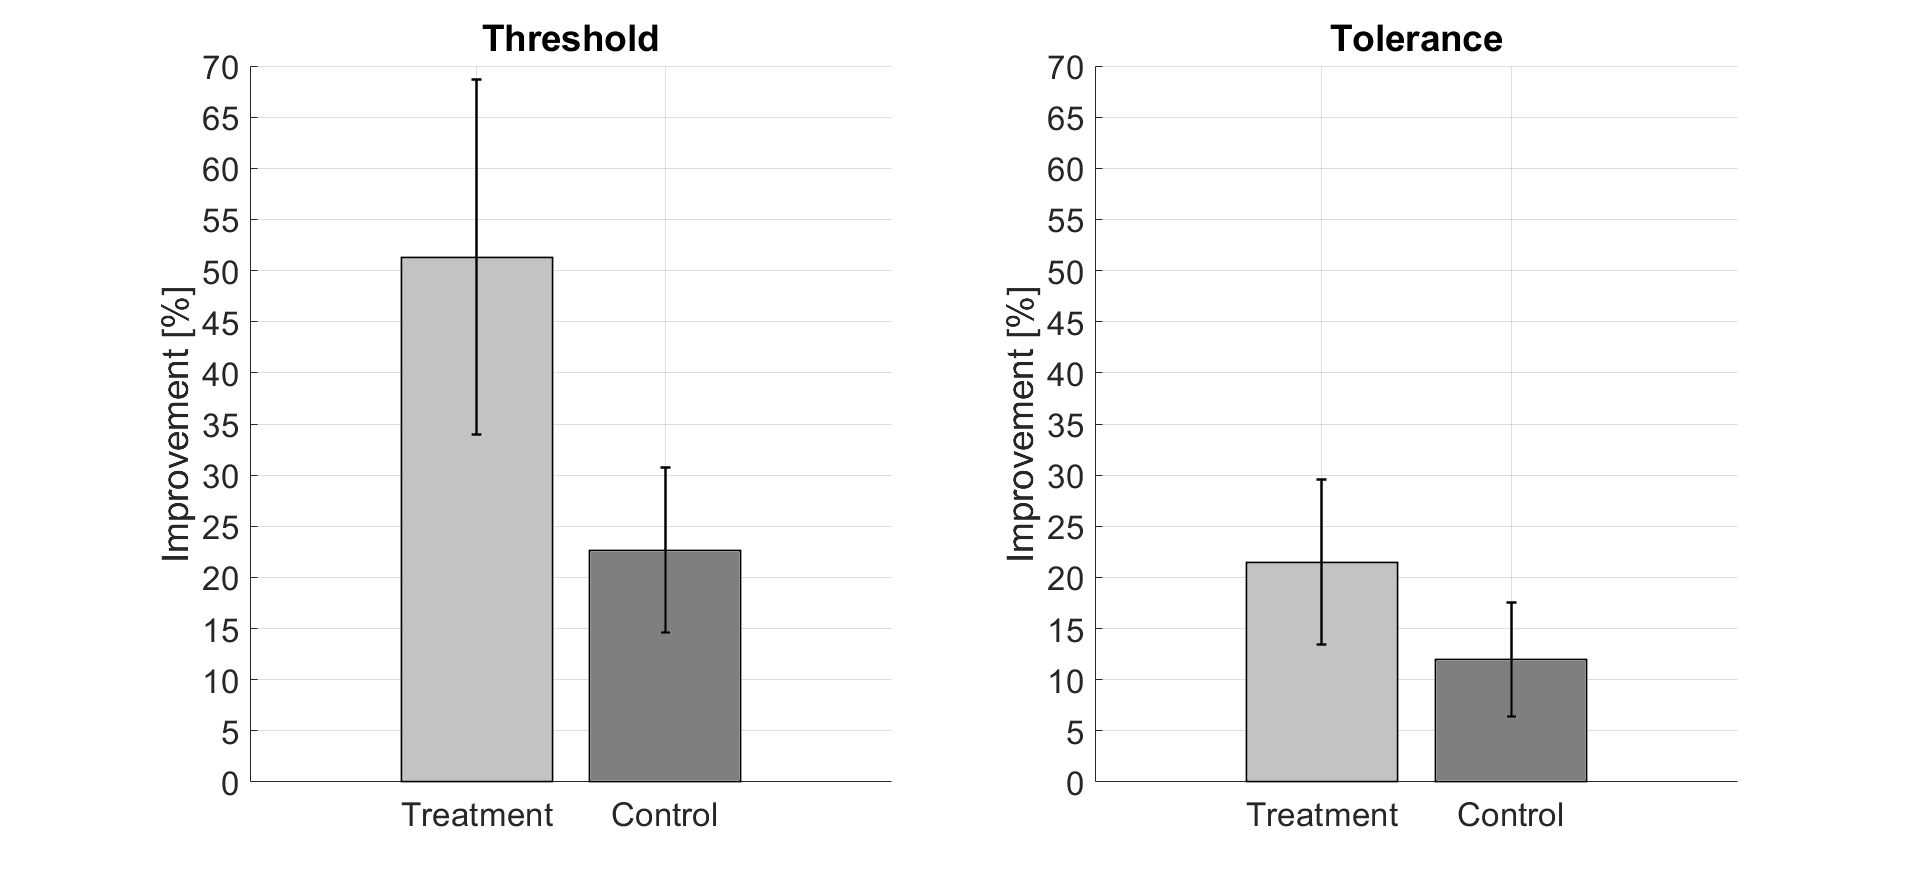
\includegraphics[width=1\textwidth]{figures/barplot.png} 
	\caption{Improvement for Threshold (left) and Tolerance (right) with associated standard error for treatment (light grey) and control group (dark grey).}
	\label{fig:barplot}  
\end{figure}

\section{Test of Normality}
The results from the Shapiro-Wilk test ($\alpha$ > 0.05), which was used to test for normality of Threshold and Tolerance, Pre and Post,  for treatment and control group, are illustrated in \tabref{tab:ShapiroWilk1}.

\begin{longtable} {l|c|c|c|c}
\caption{Shapiro-Wilk test for normality of Threshold and Tolerance, Pre and Post, for treatment and control group. P-values marked with an asterisk indicate normality.}
	\label{tab:ShapiroWilk1} \\
 \cellcolor[HTML]{C0C0C0}{} &
  \cellcolor[HTML]{C0C0C0}{\textbf{Threshold Pre}} &  \cellcolor[HTML]{C0C0C0}{\textbf{Threshold Post}} &
 \cellcolor[HTML]{C0C0C0}{\textbf{Tolerance Pre}} & \cellcolor[HTML]{C0C0C0}{\textbf{Tolerance Post}}
 \\ \hline 
%\cellcolor[HTML]{C0C0C0} & Treatment (21)& 0.173* & 0.852* & 0.149* & 0.121* \\ \cline{2-6}
%\cellcolor[HTML]{C0C0C0}{\multirow{-2}{*}{All subjects}} & Control (21)& 0.016  & 0.080* & 0.155*  & 0.514* \\ \hline
\cellcolor[HTML]{C0C0C0}{\textbf{Treatment}} & 0.377*  & 0.930* & 0.582* & 0.142* \\ \hline
\cellcolor[HTML]{C0C0C0}{\textbf{Control}} & 0.077* & 0.107* & 0.976* & 0.426* \\ \hline
\end{longtable}
\vspace{-.5cm}

The results from the Shapiro-Wilk test, which was used to test the normality of Improvement in Threshold and Tolerance, are illustrated in \tabref{tab:ShapiroWilk2}.

\begin{longtable} {l|c|c}
\caption{Shapiro-Wilk test for normality of Improvement (Imp) in Threshold and Tolerance for treatment and control group. P-values marked with an asterisk indicate normality.}
	\label{tab:ShapiroWilk2} \\
 \cellcolor[HTML]{C0C0C0}{} &
 \multicolumn{1}{c|}{ \cellcolor[HTML]{C0C0C0}{\textbf{Threshold Imp}}} & \multicolumn{1}{|c}{ \cellcolor[HTML]{C0C0C0}{\textbf{Tolerance Imp}}}  	\\ \hline
%\cellcolor[HTML]{C0C0C0} & Treatment (21) & 0.013 &  0.888* \\  \cline{2-4}
%\cellcolor[HTML]{C0C0C0}\multirow{-2}{*}{All subjects} & Control (21) & 0.233*  & 0.856*  \\ \hline
\cellcolor[HTML]{C0C0C0}{\textbf{Treatment}} & 0.197* & 0.975*  \\ \hline
\cellcolor[HTML]{C0C0C0}{\textbf{Control}} & 0.148* & 0.929* \\ \hline
\end{longtable}
\vspace{-.5cm}

\section{Test of Equality of Variance}
The results from Levene's test ($\alpha$ > 0.05), which was used to test the equality of variance of Threshold and Tolerance, Pre and Post, between treatment and control group, are illustrated in \tabref{tab:Levene1}.

\begin{longtable} {c|c|c|c}
\caption{Levene's test for equality of variance of Threshold and Tolerance, Pre and Post, between treatment and control group. P-values marked with an asterisk indicate equal variance.}
	\label{tab:Levene1} \\ 
 \cellcolor[HTML]{C0C0C0}{\textbf{Threshold Pre}} &  \cellcolor[HTML]{C0C0C0}{\textbf{Threshold Post}} 
 & \cellcolor[HTML]{C0C0C0}{\textbf{Tolerance Pre}}
 &  \cellcolor[HTML]{C0C0C0}{\textbf{Tolerance Post}}	\\ \hline 
0.437* & 0.551* & 0.354* & 0.658*\\ \hline
\end{longtable}
\vspace{-.5cm}

The results from the Levene's test, which was used to test the equality of variance of Improvement in Threshold and Tolerance between treatment and control group, are illustrated in \tabref{tab:Levene2}.

\begin{longtable} {c|c}
\caption{Levene's test for equality of variance of Improvement (Imp) in Threshold and Tolerance between treatment and control group. P-values marked with an asterisk indicate equal variance.}
	\label{tab:Levene2} \\ 
\cellcolor[HTML]{C0C0C0} {\textbf{Threshold Imp}} & \cellcolor[HTML]{C0C0C0} {\textbf{Tolerance Imp}} \\ \hline
 0.013 & 0.159 \\ \hline
\end{longtable}
\vspace{-.5cm}

\section{Two-way mixed ANOVA}
The dataset was normal distributed indicated in \tabref{tab:ShapiroWilk1}, and had an equal variance indicated in  \tabref{tab:Levene1}. Hence a two-way mixed ANOVA ($\alpha$ < 0.05) was used to test if there is a difference within and between treatment and control group. Hereby the Pre and Post measurements of Threshold and Tolerance were compared to assess the within-subjects effect. Treatment and control group were compared to assess the between-subjects effect. Results from the two-way mixed ANOVA are illustrated in \tabref{tab:ANOVA1} for Threshold and \tabref{tab:ANOVA2} for Tolerance. 

\begin{longtable} {l|l|c|c|c}
\caption{Two-way mixed ANOVA for Threshold, Pre and Post, comparing treatment and control group. P-values marked with an asterisk indicate significant difference. F-value and degree of freedom (df) are illustrated as well.}
	\label{tab:ANOVA1} \\
%\multicolumn{3}{c|}{ \cellcolor[HTML]{C0C0C0}{\textbf{Within-Subjects Effect}}} & \multicolumn{3}{c}{ \cellcolor[HTML]{C0C0C0}{\textbf{Between-Subjects Effect}}}  	\\  \rule{0pt}{3ex} 
  \cellcolor[HTML]{C0C0C0}{} &  \cellcolor[HTML]{C0C0C0}{} & \multicolumn{1}{c|}{ \cellcolor[HTML]{C0C0C0}{\textbf{df}}} &
 \multicolumn{1}{c|}{ \cellcolor[HTML]{C0C0C0}{\textbf{F-value}}} & \multicolumn{1}{c}{ \cellcolor[HTML]{C0C0C0}{\textbf{p-value}}} \\ \hline  
\cellcolor[HTML]{C0C0C0} & Measurement & 1 & 13.051 & 0.001* \\ \cline{2-5}
\cellcolor[HTML]{C0C0C0}\multirow{-2}{*}{\textbf{Within-Subjects effect}} & Measurement x Group & 1 & 0.451 & 0.507  \\ \hline
\cellcolor[HTML]{C0C0C0}{\textbf{Between-Subjects effect}} & Group & 30 & 1.492 & 0.231 \\ \hline
\end{longtable}
\vspace{-.5cm}

The test indicates that there is a significant main effect between Pre and Post of Threshold measurements (within-subject effect, Measurement), F(1,30) = 13.051, p = 0.001. However, no significant main effect is seen between treatment and control group for Threshold (between-subjects effect, Group), F(1,30) = 1.492, p = 0.231 nor a significant main interaction between measurements and group (within-subjects effect, Measurement x Group), F(1,30) = 0.451, p = 0.507. 
 
\begin{longtable} {l|l|c|c|c}
\caption{Two-way mixed ANOVA for Tolerance, Pre and Post, comparing treatment and control group. P-values marked with an asterisk indicate significant difference. F-value and degree of freedom (df) are illustrated as well.}
	\label{tab:ANOVA2} \\
%\multicolumn{3}{c|}{ \cellcolor[HTML]{C0C0C0}{\textbf{Within-Subjects Effect}}} & \multicolumn{3}{c}{ \cellcolor[HTML]{C0C0C0}{\textbf{Between-Subjects Effect}}}  	\\  \rule{0pt}{3ex} 
  \cellcolor[HTML]{C0C0C0}{} &  \cellcolor[HTML]{C0C0C0}{} & \multicolumn{1}{c|}{ \cellcolor[HTML]{C0C0C0}{\textbf{df}}} &
 \multicolumn{1}{c|}{ \cellcolor[HTML]{C0C0C0}{\textbf{F-value}}} & \multicolumn{1}{c}{ \cellcolor[HTML]{C0C0C0}{\textbf{p-value}}} \\ \hline  
\cellcolor[HTML]{C0C0C0} & Measurement & 1 & 8.918 & 0.006*  \\ \cline{2-5}
\cellcolor[HTML]{C0C0C0}\multirow{-2}{*}{\textbf{Within-Subjects effect}} & Measurement x Group & 1 & 0.532 & 0.472  \\ \hline
\cellcolor[HTML]{C0C0C0}{\textbf{Between-Subjects effect}} & Group & 30 & 3.289 & 0.080  \\ \hline
\end{longtable}
\vspace{-.5cm}

The test indicates that there is a significant main effect between Pre and Post of Tolerance measurements (within-subject effect, Measurement), F(1,30) = 8.981, p = 0.006. However, no significant main effect is seen between treatment and control group for Threshold (between-subjects effect, Group), F(1,30) = 3.289, p = 0.080 nor a significant main interaction between  measurements and group (within-subjects effect, Measurement x Group), F(1,30) = 0.532, p = 0.472. 

\section{T-test}
A normal distribution indicated in \tabref{tab:ShapiroWilk2}. Furthermore was an unequal variance seen for Threshold and an equal variance for Tolerance indicated in \tabref{tab:Levene2}, was seen for Improvement in Threshold and Tolerance for treatment and control group, thus a t-test ($\alpha$ < 0.05) was used to test if there was a difference between treatment and control group. Results from this test are illustrated in \tabref{tab:T-test1}.

\begin{longtable} {c|c|c|c}
	\caption{T-test for Threshold and Tolerance Improvement for treatment and control group. P-values marked with an asterisk indicate significant difference. F-value and degree of freedom (df) are illustrated as well.}	\label{tab:T-test1} \\
% \cellcolor[HTML]{C0C0C0}{\textbf{Threshold}} &  \cellcolor[HTML]{C0C0C0}{\textbf{Tolerance}}	\\ \hline
 \cellcolor[HTML]{C0C0C0}{}  & \cellcolor[HTML]{C0C0C0}{\textbf{df}} &  \cellcolor[HTML]{C0C0C0}{\textbf{F-value}} & \cellcolor[HTML]{C0C0C0}{\textbf{p-value}} \\ \hline  
 \cellcolor[HTML]{C0C0C0}{\textbf{Threshold}} & 19.892 & 6.967 & 0.149  \\ \hline
 \cellcolor[HTML]{C0C0C0}{\textbf{Tolerance}} & 30 & 2.084 & 0.330 \\ \hline
\end{longtable}
\vspace{-.5cm}

The test indicates that there is no significant difference in Improvement in Threshold, F(1,19.892)= 6.967, p = 0.149 and Tolerance, F(1,30)= 2.084, p = 0.330 between treatment and control group.


%\subsection{Visual inspection on the results}
%To get a visual view of the results boxplots comparing the thresholds pre and post for the control and treatment group are made (figure  \ref{fig:boxplot_thres_all}).
%
%\begin{figure}[H]                                         %   File-type can be specified
%	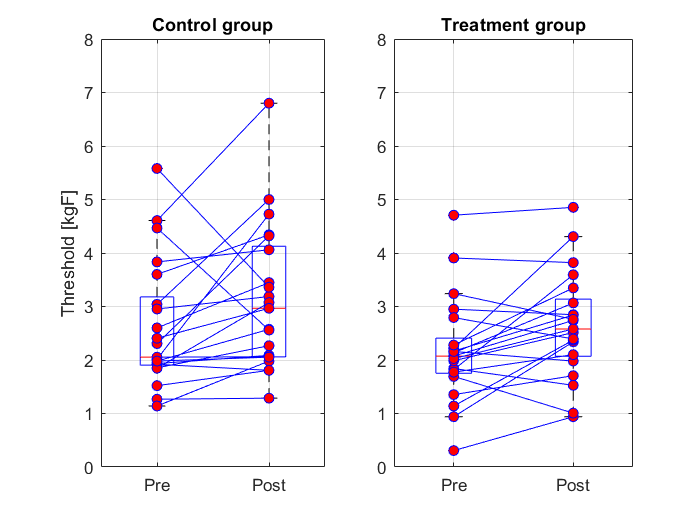
\includegraphics[width=1\textwidth]{figures/boxplot_threshold_all.PNG}  %<--but is not needed.
%	\caption{}
%	\label{fig:boxplot_thres_all}  %<--give the figure a label, so you can reference!
%\end{figure}               %   For the label to work it must be under the caption.
%
%Box plots showing the same for the tolerance is also made (figure \ref{fig:boxplot_tol_all}). 
%\begin{figure}[H]                                         %   File-type can be specified
%	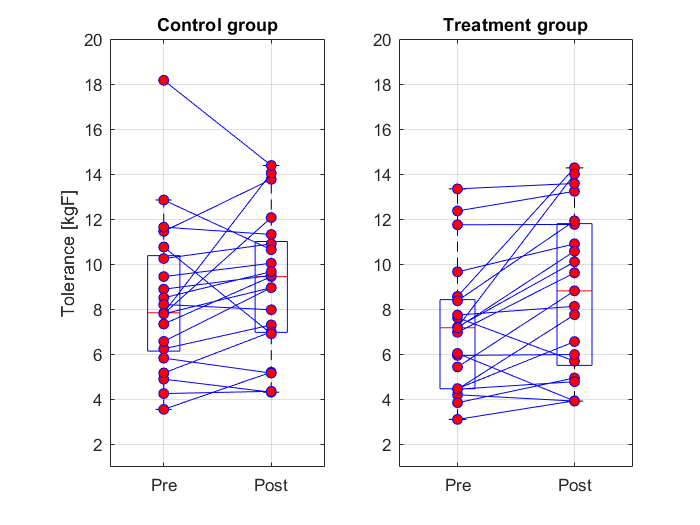
\includegraphics[width=1\textwidth]{figures/boxplot_tolerance_all.PNG}  %<--but is not needed.
%	\caption{}
%	\label{fig:boxplot_tol_all}  %<--give the figure a label, so you can reference!
%\end{figure}               %   For the label to work it must be under the caption.
%
%The mean percentage increase in the threshold and tolerance for the control and treatment are shown in figure \ref{fig:mean_increase_all}. 
% 
%\begin{figure}[H]                                         %   File-type can be specified
%	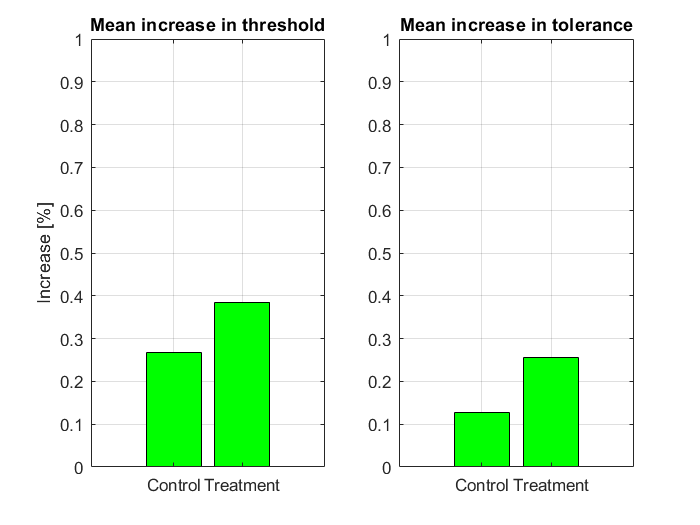
\includegraphics[width=1\textwidth]{figures/mean_increase_all.PNG}  %<--but is not needed.
%	\caption{Mean percentage increase in threshold for control and treatment group (left) and mean percentage increase in tolerance for control and treatment group (right)}
%	\label{fig:mean_increase_all}  %<--give the figure a label, so you can reference!
%\end{figure}               %   For the label to work it must be under the caption.


%\begin{longtable} {l|c|c|c|c|c|c}
%	\caption{Threshold and tolerance pre and post and the percentage difference between these values for the control group.}
%	\label{tab:Treatment} \\
%\cellcolor[HTML]{C0C0C0} {} & 
%\multicolumn{3}{c|}{ \cellcolor[HTML]{C0C0C0}{\textbf{Threshold}}} & \multicolumn{3}{c}{ \cellcolor[HTML]{C0C0C0}{\textbf{Tolerance}}}  	\\  \rule{0pt}{3ex} 
%% \rowcolor[HTML]{C0C0C0} \color[HTML]{000000}{} & 
%% \multicolumn{3}{c|}{ \color[HTML]{000000}{\textbf{Threshold}}} & \multicolumn{3}{c}{ \color[HTML]{000000}{\textbf{Tolerance}}}  	\\  \rule{0pt}{3ex} 
%  \cellcolor[HTML]{C0C0C0}{} &
% \multicolumn{1}{c|}{ \cellcolor[HTML]{C0C0C0}{Pre [KgF]}} & \multicolumn{1}{c|}{ \cellcolor[HTML]{C0C0C0}{Post [KgF]}} 
% & \multicolumn{1}{c}{ \cellcolor[HTML]{C0C0C0}{\textcolor[HTML]{C0C0C0}{0}Diff [\%]\textcolor[HTML]{C0C0C0}{0}}}
% & \multicolumn{1}{|c|}{ \cellcolor[HTML]{C0C0C0}{Pre [KgF]}} 
% & \multicolumn{1}{c|}{ \cellcolor[HTML]{C0C0C0}{Post [KgF]}} 
% & \multicolumn{1}{c}{ \cellcolor[HTML]{C0C0C0}{\textcolor[HTML]{C0C0C0}{0}Diff [\%]\textcolor[HTML]{C0C0C0}{0}}}  	\\ \hline 
%\#T1 & 1.84 & 1.53 & -17.03 & 4.21 & 3.93 & -6.66 \\ \hline
%\#T2 & 2.95 & 2.85  & -3.50 & 7.63  & 5.70 & -25.26 \\ \hline
%\#T3 & 2.13 & 3.07 & 43.75 & 7.75 & 8.13 & 4.99 \\ \hline
%\#T4 & 0.94 & 2.34  & 148.94  & 3.85 & 4.95 & 28.55 \\ \hline
%\#T5 & 1.35 & 1.71  & 26.11 & 3.11 & 3.94 & 26.55 \\ \hline	
%\#T6 & 0.31 & 0.94   & 206.52 & 5.95 & 5.99 & 0.67 \\ \hline
%\#T7 & 2.07 & 2.74  & 32.15 & 5.44 & 8.82 & 62.13 \\ \hline
%\#T8 & 1.82 & 3.59 & 97.44 & 7.21 & 10.11 & 40.11 \\ \hline
%\#T9 & 2.17 & 2.84  & 31.08 & 6.98 & 9.62 & 37.82 \\ \hline
%%\#T10 & 4.71 & 4.85  & 3.12 & 12.37*  & 13.24* & 7.06 \\ \hline
%\#T11 & 2.22 & 4.31 & 93.99 & 4.45 & 7.76 & 74.25 \\ \hline
%\#T12 & 1.99 & 2.51 & 26.51 & 4.45 & 4.79 & 7.49 \\ \hline
%\#T13 & 1.14 & 2.37 & 108.19 & 4.48 & 6.57 & 46.58 \\ \hline
%\#T14 & 1.69 & 1.01 & -40.55 & 6.04 & 3.93 & -34.88 \\ \hline
%%\#T15 & 2.03 & 2.58 & 27.30 & 8.57* & 14.28* & 66.56 \\ \hline
%%\#T16 & 2.79 & 2.39 & -14.32 & 13.35* & 13.59* & 1.80 \\ \hline
%%\#T17 & 3.24 & 2.76 & -14.81 & 11.75 & 11.77* & 0.11 \\ \hline
%%\#T18 & 2.16 & 1.98 & -8.33 & 8.38* & 11.93* & 42.32 \\ \hline
%\#T19 & 1.77 & 2.10 & 18.42 & 9.66 & 10.91 & 12.87  \\ \hline
%%\#T20 & 2.28 & 3.35 & 46.78 & 7.20  & 14.01* & 94.54 \\ \hline
%\#T21 & 3.91 &  3.82 & -2.22 & 7.18 & 10.58 & 47.35 \\ \hline
%Mean &   &   &  & & & \\  \hline
%\end{longtable}

%\begin{longtable} {l|c|c|c|c|c|c}
%	\caption{Threshold and tolerance pre and post and the percentage difference between these values for the control group.}
%	\label{tab:Control} \\
%% \rowcolor[HTML]{C0C0C0} 
%%  \color[HTML]{000000}{} & 
%% \multicolumn{3}{c|}{ \color[HTML]{000000}{\textbf{Threshold}}} & \multicolumn{3}{c}{ \color[HTML]{000000}{\textbf{Tolerance}}}  	\\  \rule{0pt}{3ex} 
%\cellcolor[HTML]{C0C0C0} {} & 
%\multicolumn{3}{c|}{ \cellcolor[HTML]{C0C0C0}{\textbf{Threshold}}} & \multicolumn{3}{c}{ \cellcolor[HTML]{C0C0C0}{\textbf{Tolerance}}}  	\\  \rule{0pt}{3ex} 
%  \cellcolor[HTML]{C0C0C0}{} &
% \multicolumn{1}{c|}{ \cellcolor[HTML]{C0C0C0}{Pre [KgF]}} & \multicolumn{1}{c|}{ \cellcolor[HTML]{C0C0C0}{Post [KgF]}} 
% & \multicolumn{1}{c}{ \cellcolor[HTML]{C0C0C0}{\textcolor[HTML]{C0C0C0}{0}Diff [\%]\textcolor[HTML]{C0C0C0}{0}}}
% & \multicolumn{1}{|c|}{ \cellcolor[HTML]{C0C0C0}{Pre [KgF]}} 
% & \multicolumn{1}{c|}{ \cellcolor[HTML]{C0C0C0}{Post [KgF]}} 
% & \multicolumn{1}{c}{ \cellcolor[HTML]{C0C0C0}{\textcolor[HTML]{C0C0C0}{0}Diff [\%]\textcolor[HTML]{C0C0C0}{0}}}  	\\ \hline   
%\#C1 & 3.04	& 5.00	&	64.47	& 7.80	& 	12.07 &	54.79\\ \hline
%\#C2 & 1.85 	& 2.27	&	22.30	& 7.35	& 	9.45 & 28.68	\\ \hline
%\#C3 & 1.92 	& 1.81	&	-5.90	& 4.90	& 	4.32 & -11.84	\\ \hline
%\#C4 & 1.93 	& 2.09	&	7.93		& 6.25	&	7.31 & 16.97	\\ \hline
%%\#C5 & 2.01 	& 4.73 	& 	134.77	& 11.46* 	& 13.77* & 20.19		\\ \hline
%%\#C6 & 2.60 	& 3.45	& 	32.56		& 7.85*	& 14.05 & 79.01		\\ \hline	
%\#C7 & 3.60 & 4.34	& 	20.56		& 6.57 & 8.96  &	36.31 \\ \hline
%\#C8 & 1.98 & 2.57	& 	29.97		& 10.25	& 10.91 &	6.37	\\ \hline
%\#C9 & 2.59 & 3.19 	& 	7.9		& 8.89	& 9.51 & 6.90		\\ \hline
%%\#C10 & 4.61 & 6.80	& 	47.61		& 12.85*	& 10.65* & -17.17 \\ \hline
%\#C11 & 1.27 & 1.29 	& 	1.58		& 3.56	& 5.21 &  46.25\\ \hline
%\#C12 & 2.31 & 4.32 	& 	87.28	& 9.45 & 10.05 & 6.28 \\ \hline
%\#C13 & 4.47 & 2.56 	& 	-42.69	& 8.51 & 9.67 & 13.67 \\ \hline
%\#C14 & 1.85 & 3.07 & 	66.43	 & 5.17 & 7.00 & 35.31 \\ \hline
%\#C15 & 1.14 & 1.98 & 	73.68 & 5.83 & 5.17 & -11.43 \\ \hline
%\#C16 & 2.05 & 2.06 & 	0.32 & 8.21 & 7.98 & -2.84 \\ \hline
%\#C17 & 1.52 & 1.81 &	18.86 & 10.77 & 6.91 & -35.79 \\ \hline
%\#C18 & 1.98 & 2.05 & 	3.70 & 4.26  &  4.36 & 2.35 \\ \hline
%%\#C19 & 5.58 & 2.36 & 	-39.78 & 18.17* & 14.39* & -20.81 \\ \hline
%\#C20 & 2.41 & 2.97 &  23.27 & 7.80 &  8.96 & 14.87\\ \hline
%\#C21 & 3.83 & 4.06 & 5.91  & 11.65 & 11.32 & -2.78 \\ \hline
%Mean &   &   &  & & & \\  \hline
%\end{longtable}


%************* KRUSKAL *****************
%\subsection{Kruskal-Wallis test}
%A normal distribution was not seen in every group of the treatment and control, why a non-parametric test, Kruskall Wallis ($\alpha$ < 0.05), was used to test if there is a  difference between the groups. Results from this test are illustrated in \tabref{tab:KruskalWallis1}.
%
%\begin{longtable} {l|c|c|c|c}
%	\caption{Kruskal-Wallis Test for threshold and tolerance difference for treatment and control respectively. The asterisk indicates normality.}
%	\label{tab:KruskalWallis1} \\ 
%	 \cellcolor[HTML]{C0C0C0} {} &
%\multicolumn{2}{c|}{ \cellcolor[HTML]{C0C0C0}{\textbf{Threshold}}} & \multicolumn{2}{c}{ \cellcolor[HTML]{C0C0C0}{\textbf{Tolerance}}}  	\\  \rule{0pt}{3ex} 
%  \cellcolor[HTML]{C0C0C0}{} &
% \multicolumn{1}{c|}{ \cellcolor[HTML]{C0C0C0}{Pre }} & \multicolumn{1}{c|}{ \cellcolor[HTML]{C0C0C0}{Post}} 
% & \multicolumn{1}{|c|}{ \cellcolor[HTML]{C0C0C0}{Pre}} 
% & \multicolumn{1}{c}{ \cellcolor[HTML]{C0C0C0}{Post}} 	\\ \hline
%% \rowcolor[HTML]{C0C0C0}  \color[HTML]{000000}{} & 
%%   \color[HTML]{000000}{\textbf{Treshold Pre}} & 
%%  \color[HTML]{000000}{\textbf{Threshold Post}} & 
%%   \color[HTML]{000000}{\textbf{Tolerance Pre}} & 
%%\color[HTML]{000000}{\textbf{Tolerance Post}}  
%% \\ \hline
%Subject (42) & 0.327  & 0.352 & 0.155  & 0.669 \\ \hline
%\end{longtable}
%\vspace{-.5cm}
%
%There is no significant difference between the threshold and tolerance pre and post.

%************* MANN-WHITNEY U Test ***************
%\subsection{Mann-Whitney U Test}
%A normal distribution was not seen between all the threshold and tolerance difference, why a Mann-Whitney U ($\alpha$ < 0.05) was used to test if there exists a difference between the groups. Results from this test are illustrated in \tabref{tab:MannWhitney1}.
%
%\begin{longtable} {l|c|c}
%	\caption{Mann-Whitney U test for threshold and tolerance difference for treatment and control respectively.}	\label{tab:MannWhitney1} \\ 
% \cellcolor[HTML]{C0C0C0} {} & 
% \multicolumn{1}{c|}{ \cellcolor[HTML]{C0C0C0}{\textbf{Threshold}}} & \multicolumn{1}{c}{ \cellcolor[HTML]{C0C0C0}{\textbf{Tolerance}}}  	\\  \rule{0pt}{3ex} 
%  \cellcolor[HTML]{C0C0C0}{} &
% \multicolumn{1}{c|}{ \cellcolor[HTML]{C0C0C0}{Difference }} & \multicolumn{1}{|c}{ \cellcolor[HTML]{C0C0C0}{Difference}}  	\\ \hline
%% \rowcolor[HTML]{C0C0C0}  \color[HTML]{000000}{} & 
%%   \color[HTML]{000000}{\textbf{Treshold Difference}} &  \color[HTML]{000000}{\textbf{Tolerance Difference}}  
%% \\ \hline
%Subject (42) & 0.850 & 0.195 \\ \hline
%\end{longtable}
%\vspace{-.5cm}
%
%The test indicates that there is no significant difference between the difference in threshold and tolerance.